\chapter{Analyse}\label{sec:analyse}

\section{Systemsekvensdiagram}
\todo{write stuff about SSD}
\begin{figure}
    \centering
    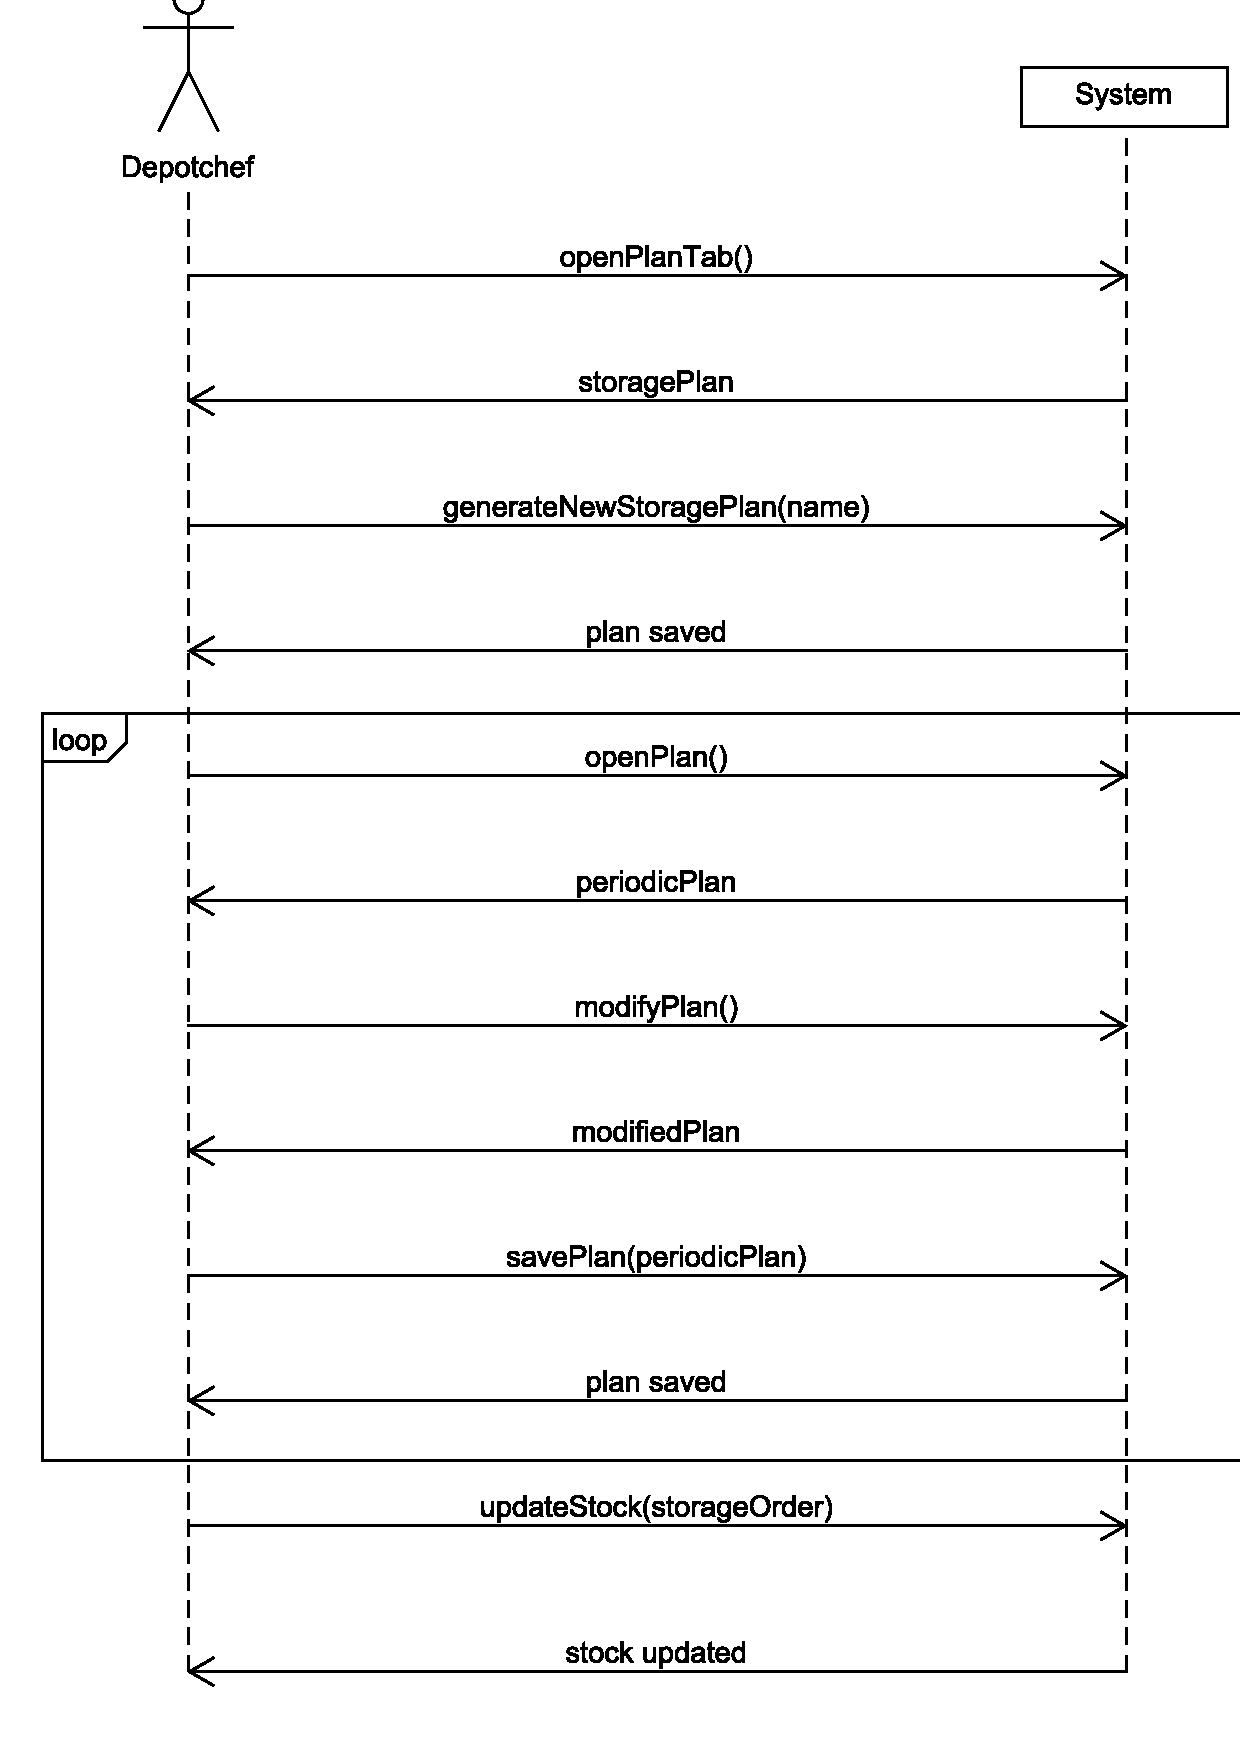
\includegraphics[width=50mm,scale=0.5]{figures/analyse/SSD.png}
    \caption{Systemsekvensdiagram}
    \label{fig:ssd}
\end{figure}


\section{Operationskontrakt}
\todo{write stuff about operationskontrakt}
%remember to talk about the autogeneration continuation process thing algorithm stuff :) 

\begin{center}
    \begin{longtable}{ |p{360pt}| }
        \hline
        \textbf{Operationskontrakt}
        \\
        \noindent\fbox{%
            \parbox{4.88in}{%
                \textbf{Operation:} openPlanTab() \\ Åbner planfanen i programmet
                
            }%
        }

        \noindent\fbox{%
            \parbox{4.88in}{%
                \textbf{Operation:} generateNewStoragePlan(name) \\ 
                Use Case: Bestil Varer \\

                Præ-betingelser: en instans af productMap eksisterer \\

                Post-betingelser: \\
                - sp.name blev sat til name \\
                - En instans af PeriodicPlan blev oprettet \\
                - pp.period blev sat til period \\
                - en instans af sOrder blev oprettet \\
                - pp blev associeret med product og sOrder \\
                - p blev associeret med supplier og productLine \\
                - sOrder blev associeret med supplier og productLine 
            }%
        }

        \noindent\fbox{%
            \parbox{4.88in}{%
                \textbf{Operation:} openPlan() \\
                Den generede plan åbnes i planfanen i programmet
            }%
        }
        
        \noindent\fbox{%
            \parbox{4.88in}{%
                \textbf{Operation:} savePlan(periodicPlan) \\
                Use Case: CRUD StoragePlan \\
                Præ-betingelser: En instans af StoragePlan eksisterer \\
                Post-betingelser: \\
                - De nye periodicPlan instanser gemmes i periodicPlans
            }%
        }

        \noindent\fbox{%
            \parbox{4.88in}{%
                \textbf{Operation:} updateStock(storageOrder)
                Use Case: Modtag Varer \\
                Præ-betingelser: Produkterne bestilt fra en storageOrder er ankommet til depotet. \\
                Post-betingelser: \\
                -

            }%
        }
        
    \end{longtable}
\end{center}